
\begin{frame}
	\frametitle{Overview}
	\begin{columns}
		\column{0.55\textwidth}
		We have four Wien settings:
		\begin{itemize}
			\item[\textbullet] 1) VWien = $0.0^\circ$, no flip
			\item[\textbullet] 2) VWien = $+90.0^\circ$, flip right
			\item[\textbullet] 3) VWien = $-90.0^\circ$, flip right
			\item[\textbullet] 4) VWien = $+90.0^\circ$, flip left
		\end{itemize}
		\column{0.55\textwidth}
		\begin{figure}
			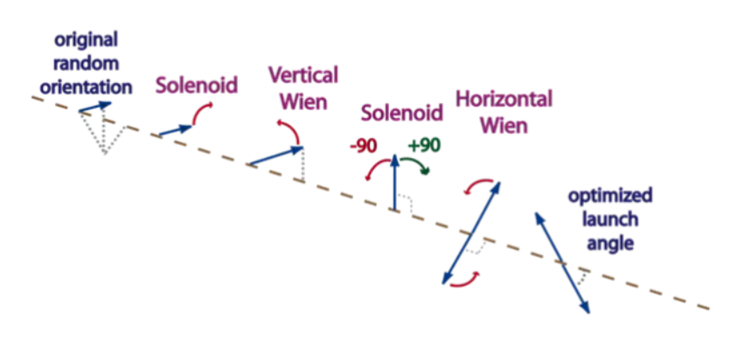
\includegraphics[width=65mm]{./Figs/Wien.png}
		\end{figure}
	\end{columns}
	\vspace{5mm}
	\textbf{Goal}: We want to do a PITA scan, position scan, and RHWP study for all four Wien settings.
		
\end{frame}